\documentclass{article}

% content/resources/templates/preamble.tex
\usepackage[margin=0.6in]{geometry}
\author{Milav Dabgar}
\usepackage{amsmath,amssymb,amsthm}
\usepackage{booktabs}
\usepackage{multirow}
\usepackage{xcolor}
\usepackage{tcolorbox}
\tcbuselibrary{breakable,skins}
\usepackage[colorlinks=true,linkcolor=blue]{hyperref}
\usepackage{titlesec}
\usepackage{enumitem}
\usepackage{tikz}
\usepackage{pgfplots}
\usepackage{circuitikz}
\usepackage[version=4]{mhchem}
\usepackage{longtable}
\usepackage{array}
\usepackage{float}
\usepackage{caption}
\usepackage{listings}

\lstset{
  basicstyle=\small\ttfamily,
  breaklines=true,
  breakatwhitespace=false,
  postbreak=\mbox{\textcolor{red}{$\hookrightarrow$}\space},
  float=false,
  numbers=left,
  numberstyle=\tiny\color{gray},
  numbersep=10pt,
  xleftmargin=2em,
  keywordstyle=\color{blue},
  commentstyle=\color{green!60!black},
  stringstyle=\color{purple},
  backgroundcolor=\color{gray!5},
  showstringspaces=false,
  tabsize=2,
  captionpos=b,
  keepspaces=true,
  columns=flexible
}

\pgfplotsset{compat=1.18}
\usetikzlibrary{shapes,arrows,positioning,calc,patterns,decorations.pathmorphing,decorations.markings,arrows.meta}

% Color scheme
\definecolor{headcolor}{RGB}{0,102,204}
\definecolor{keycolor}{RGB}{220,20,60}
\definecolor{solutioncolor}{RGB}{34,139,34}
\definecolor{mnemoniccolor}{RGB}{148,0,211}
\definecolor{codecolor}{RGB}{0,0,100}

% Spacing
\setlength{\parskip}{3pt}
\setlist[itemize]{nosep}
\setlist[enumerate]{nosep}

% Title formatting
\titleformat{\section}{\Large\bfseries\color{headcolor}}{\thesection}{1em}{}
\titleformat{\subsection}{\large\bfseries\color{headcolor}}{\thesubsection}{1em}{}

% Pandoc tightlist compatibility
\providecommand{\tightlist}{%
  \setlength{\itemsep}{0pt}\setlength{\parskip}{0pt}}

% Pandoc longtable compatibility
\newcounter{none}
\def\thenone{}


% content/resources/templates/english-boxes.tex

% Custom environments
\newtcolorbox{solutionbox}{
 breakable,
 enhanced,
 colback=solutioncolor!5!white,
 colframe=solutioncolor!75!black,
 fonttitle=\bfseries,
 title=Solution
}

\newtcolorbox{solutionboxnobreak}{
 colback=solutioncolor!5!white,
 colframe=solutioncolor!75!black,
 fonttitle=\bfseries,
 title=Solution
}

\newtcolorbox{keyformula}{
 breakable,
 enhanced,
 colback=keycolor!5!white,
 colframe=keycolor!75!black,
 fonttitle=\bfseries,
 title=Key Formula
}

\newtcolorbox{mnemonicboxenv}{
 breakable,
 enhanced,
 colback=mnemoniccolor!5!white,
 colframe=mnemoniccolor!75!black,
 fonttitle=\bfseries,
 title=Mnemonic
}

\newcommand{\mnemonicbox}[1]{%
  \begin{mnemonicboxenv}
    #1
  \end{mnemonicboxenv}
}


% Custom commands for GTU solutions
% This file defines semantic commands for consistent formatting

% Question command with automatic formatting
\newcommand{\question}[2]{%
  \section*{Question #1}%
  \textbf{#2}%
}

% OR question variant
\newcommand{\questionor}[2]{%
  \section*{Question #1 OR}%
  \textbf{#2}%
}

% Proper table environment with caption
\newenvironment{answertable}[1]{%
  \begin{table}[htbp]
  \centering
  \caption{#1}
}{%
  \end{table}
}

% Proper figure environment for diagrams
\newenvironment{answerdiagram}[1]{%
  \begin{figure}[htbp]
  \centering
  \caption{#1}
}{%
  \end{figure}
}

% Semantic markup for key terms
\newcommand{\keyword}[1]{\textbf{#1}}
\newcommand{\code}[1]{\texttt{#1}}
\newcommand{\classname}[1]{\texttt{#1}}
\newcommand{\methodname}[1]{\texttt{#1}}

% Proper quotation marks
\newcommand{\mnemonic}[1]{``#1''}


\title{Electronics Devices \& Circuits (1323202) - Summer 2023 Solution}
\date{July 31, 2023}

\begin{document}
\maketitle

\questionmarks{1(a)}{3}{Draw the symbol of (1)SCR (2)Diac(3)Triac}

\begin{solutionbox}
\begin{center}
\begin{circuitikz}[american, scale=1.2, transform shape]
    % SCR
    \draw (0,2) to[thyristor, n=scr] (0,0);
    \node at (0, 2.5) {\textbf{SCR}};
    \node at (0, 2) [left] {A};
    \node at (0, 0) [left] {K};
    \node at (scr.gate) [right] {G};

    % DIAC (Manual drawing as to[diac] missing)
    \node at (4, 2.5) {\textbf{DIAC}};
    \draw (4, 2) -- (4, 1.6);
    \draw (4, 0.4) -- (4, 0);
    \draw (3.6, 1.6) -- (4.4, 1.6) -- (4, 0.8) -- (3.6, 1.6); % Down
    \draw (3.6, 0.8) -- (4.4, 0.8) -- (4, 1.6) -- (3.6, 0.8); % Up
    \draw (3.6, 0.8) -- (4.4, 0.8); % Bottom line of Up triangle
    \node at (4, 2) [left] {A1};
    \node at (4, 0) [left] {A2};

    % TRIAC
    \draw (8,2) to[triac, n=triac] (8,0);
    \node at (8, 2.5) {\textbf{TRIAC}};
    \node at (8, 2) [left] {MT2};
    \node at (8, 0) [left] {MT1};
    \node at (triac.gate) [right] {G};
\end{circuitikz}
\end{center}

\begin{itemize}
    \item \textbf{SCR (Silicon Controlled Rectifier)}: Three-terminal device with Anode, Cathode, and Gate
    \item \textbf{DIAC (Diode AC switch)}: Two-terminal bidirectional device with terminals A1 and A2 
    \item \textbf{TRIAC (Triode AC switch)}: Three-terminal bidirectional device with MT1, MT2, and Gate
\end{itemize}

\begin{mnemonicbox}AGK for SCR, AA for DIAC, MMG for TRIAC\end{mnemonicbox}
\end{solutionbox}

\questionmarks{1(b)}{4}{Explain the term(1) CMRR (2) Slew rate}

\begin{solutionbox}
\begin{center}
\captionof{table}{Op-Amp Parameters}
\begin{tabulary}{\linewidth}{|L|L|L|}
\hline
\textbf{Parameter} & \textbf{Definition} & \textbf{Significance} \\
\hline
\textbf{CMRR (Common Mode Rejection Ratio)} & Ratio of differential gain to common mode gain expressed in dB & Higher CMRR means better rejection of common input signals \\
\hline
\textbf{Slew Rate} & Maximum rate of change of output voltage (V/$\mu$s) & Determines how fast op-amp responds to rapidly changing inputs \\
\hline
\end{tabulary}
\end{center}

\begin{itemize}
    \item \textbf{CMRR formula}: CMRR = 20 log$_{10}$(Ad/Acm) dB
    \item \textbf{Slew Rate importance}: Affects high-frequency performance and prevents distortion
\end{itemize}

\begin{mnemonicbox}Common Mode Rejected Rapidly, Slew shows Signal Speed\end{mnemonicbox}
\end{solutionbox}

\questionmarks{1(c)}{7}{Draw and explain summing amplifier.}

\begin{solutionbox}
\begin{center}
\begin{circuitikz}[american]
    \draw (5,0) node[op amp] (opamp) {};
    
    % Feedback
    \draw (opamp.-) -- ++(0,1.5) coordinate (tmp) to[R, l=$R_f$] (tmp -| opamp.out) -- (opamp.out);
    
    % Summing Point
    \draw (opamp.-) -- ++(-0.5,0) coordinate (sumpoint);
    
    % Inputs
    \draw (sumpoint) -- ++(0,1.5) coordinate (b1) to[R, l=$R_1$, -o] ++(-2.5,0) node[left] {$V_1$};
    \draw (sumpoint) to[R, l=$R_2$, -o] ++(-2.5,0) node[left] {$V_2$};
    \draw (sumpoint) -- ++(0,-1.5) coordinate (b3) to[R, l=$R_3$, -o] ++(-2.5,0) node[left] {$V_3$};
    
    % Ground
    \draw (opamp.+) -- ++(0,-0.5) node[ground] {};
    
    % Output
    \draw (opamp.out) to[short, -o] ++(1,0) node[right] {$V_{out}$};
\end{circuitikz}
\end{center}

\textbf{Operation of Summing Amplifier:}

\begin{itemize}
    \item \textbf{Circuit function}: Adds multiple input voltages with scaling
    \item \textbf{Output equation}: Vout = -(Rf/R1 $\times$ V1 + Rf/R2 $\times$ V2 + Rf/R3 $\times$ V3)
    \item \textbf{Inverting configuration}: Input signals undergo 180$^\circ$ phase shift
    \item \textbf{Gain control}: Rf/Rn determines weight of each input signal
    \item \textbf{Application}: Audio mixing, analog computation, signal processing
    \item \textbf{Key feature}: Virtual ground at inverting input simplifies analysis
\end{itemize}

\begin{mnemonicbox}Sum with Weights: Vout = -Rf(V1/R1 + V2/R2 + V3/R3)\end{mnemonicbox}
\end{solutionbox}

\vspace{0.5em}\centerline{\textbf{OR}}\questionmarks{1(c)}{7}{Draw and explain DA converter}

\begin{solutionbox}
\begin{center}
\begin{tikzpicture}[gtu block]
    \node (d0) {D0 (LSB)};
    \node (d1) [below=0.5cm of d0] {D1};
    \node (d2) [below=0.5cm of d1] {D2};
    \node (d3) [below=0.5cm of d2] {D3 (MSB)};
    
    \node (sum) [draw, circle, minimum size=1.5cm, right=3cm of d1] {$\Sigma$};
    
    \draw [gtu arrow] (d0) -- node[above] {$2^0 R$} (sum);
    \draw [gtu arrow] (d1) -- node[above] {$2^1 R$} (sum);
    \draw [gtu arrow] (d2) -- node[below] {$2^2 R$} (sum);
    \draw [gtu arrow] (d3) -- node[below] {$2^3 R$} (sum);
    
    \node (out) [right=1.5cm of sum] {Vout};
    \draw [gtu arrow] (sum) -- (out);
\end{tikzpicture}
\end{center}

\textbf{R-2R Ladder DAC Operation:}

\begin{itemize}
    \item \textbf{Function}: Converts digital binary input to analog output voltage
    \item \textbf{Working principle}: Weighted resistor network creates scaled currents
    \item \textbf{Binary weighting}: Each bit contributes voltage proportional to its position ($2^n$)
    \item \textbf{Resolution}: Determined by number of bits (N) as $1/2^N$ of full scale
    \item \textbf{Advantages}: Simple design, good accuracy, fast conversion
    \item \textbf{Applications}: Audio equipment, signal generation, control systems
\end{itemize}

\begin{mnemonicbox}Digital Bits to Analog Steps - R-2R makes the magic\end{mnemonicbox}
\end{solutionbox}

\questionmarks{2(a)}{3}{Describe thermal run away of transistor.}

\begin{solutionbox}
\begin{center}
\begin{tikzpicture}[gtu state, node distance=3cm]
    \node (temp) [draw, rectangle, rounded corners] {Increased Temperature};
    \node (curr) [draw, rectangle, rounded corners, below right=of temp] {Increased Collector Current};
    \node (power) [draw, rectangle, rounded corners, below left=of curr] {More Power Dissipation};
    
    \draw [gtu arrow] (temp) -| (curr);
    \draw [gtu arrow] (curr) -- (power);
    \draw [gtu arrow] (power) -| (temp);
\end{tikzpicture}
\end{center}

\textbf{Thermal Runaway Process:}

\begin{itemize}
    \item \textbf{Definition}: Self-accelerating process where transistor heats up and draws more current
    \item \textbf{Cause}: Negative temperature coefficient of base-emitter voltage
    \item \textbf{Prevention}: Use proper heat sink and stabilization circuits
\end{itemize}

\begin{mnemonicbox}Heat feeds Current feeds Heat - a dangerous loop\end{mnemonicbox}
\end{solutionbox}

\questionmarks{2(b)}{4}{Draw and explain voltage series negative feedback.}

\begin{solutionbox}
\begin{center}
\begin{tikzpicture}[gtu block]
    \node (amp) [draw, rectangle, minimum width=2cm, minimum height=1cm] {Amplifier (A)};
    \node (beta) [draw, rectangle, minimum width=2cm, minimum height=1cm, below=1cm of amp] {Feedback ($\beta$)};
    \node (mix) [draw, circle, left=1cm of amp] {$\Sigma$};
    
    \draw [gtu arrow] (mix) -- (amp);
    \draw [gtu arrow] (amp) -- node[above] {Vout} +(3,0);
    \draw [gtu arrow] (amp.east) ++(1.5,0) |- (beta);
    \draw [gtu arrow] (beta) -| node[left] {Vf} (mix);
    \draw [gtu arrow] (mix.west) ++(-1,0) -- node[above] {Vin} (mix);
    
    \node at (mix) [below right] {-};
    \node at (mix) [above left] {+};
\end{tikzpicture}
\end{center}

\textbf{Voltage Series Negative Feedback:}

\begin{center}
\captionof{table}{Feedback Effects}
\begin{tabulary}{\linewidth}{|L|L|}
\hline
\textbf{Parameter} & \textbf{Effect of Negative Feedback} \\
\hline
\textbf{Gain stability} & Improved, less dependent on amplifier parameters \\
\hline
\textbf{Bandwidth} & Increased proportional to feedback factor \\
\hline
\textbf{Distortion} & Reduced significantly \\
\hline
\textbf{Input impedance} & Increased \\
\hline
\end{tabulary}
\end{center}

\begin{itemize}
    \item \textbf{Working principle}: Output voltage is sampled and fed back to input
    \item \textbf{Gain formula}: Closed-loop gain = Open-loop gain/(1 + $\beta$A)
\end{itemize}

\begin{mnemonicbox}Series says Sample Voltage, Stabilize Gain\end{mnemonicbox}
\end{solutionbox}

\questionmarks{2(c)}{7}{Draw and explain DC load line for common emitter amplifier.}

\begin{solutionbox}
\begin{center}
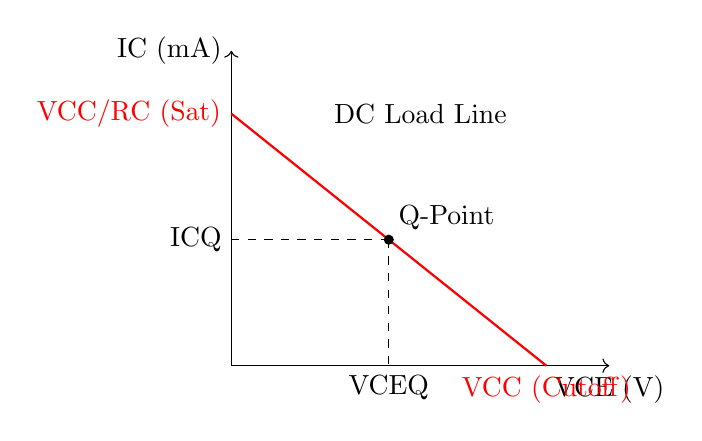
\begin{tikzpicture}[scale=0.8]
    \draw[->] (0,0) -- (0,5) node[left] {IC (mA)};
    \draw[->] (0,0) -- (6,0) node[below] {VCE (V)};
    
    % Load line
    \draw [thick, red] (0, 4) node[left] {VCC/RC (Sat)} -- (5, 0) node[below] {VCC (Cutoff)};
    
    % Q point
    \filldraw (2.5, 2) circle (2pt) node[above right] {Q-Point};
    \draw [dashed] (2.5, 2) -- (2.5, 0) node[below] {VCEQ};
    \draw [dashed] (2.5, 2) -- (0, 2) node[left] {ICQ};
    
    \node at (3, 4) {DC Load Line};
\end{tikzpicture}
\end{center}

\textbf{DC Load Line Characteristics:}

\begin{itemize}
    \item \textbf{Definition}: Graphical representation of all possible operating points
    \item \textbf{Equation}: IC = VCC/RC - VCE/RC
    \item \textbf{Key points}:
      \begin{itemize}
        \item Saturation point (VCE $\approx$ 0V, IC = VCC/RC)
        \item Cutoff point (IC $\approx$ 0mA, VCE = VCC)
        \item Q-point (selected operating point for amplification)
      \end{itemize}
    \item \textbf{Significance}: Determines biasing stability and output signal limits
    \item \textbf{Relationship}: DC load line is fixed by circuit components (VCC and RC)
\end{itemize}

\begin{mnemonicbox}Connect Cutoff to Saturation for DC Load Line\end{mnemonicbox}
\end{solutionbox}

\vspace{0.5em}\centerline{\textbf{OR}}\questionmarks{2(a)}{3}{Explain operating point(Q-point) in transistor}

\begin{solutionbox}
\begin{center}
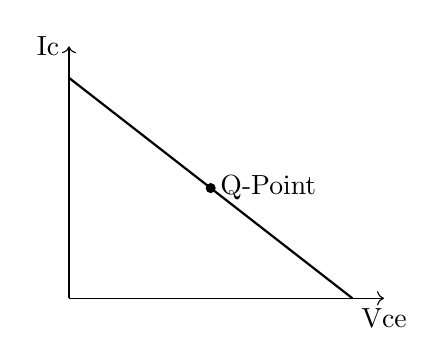
\begin{tikzpicture}[scale=0.8]
    \draw[->] (0,0) -- (0,4) node[left] {Ic};
    \draw[->] (0,0) -- (5,0) node[below] {Vce};
    \draw [thick] (0,3.5) -- (4.5,0);
    \filldraw (2.25, 1.75) circle (2pt) node[right] {Q-Point};
\end{tikzpicture}
\end{center}

\textbf{Q-Point (Operating Point):}

\begin{itemize}
    \item \textbf{Definition}: Specific DC bias point where transistor operates in active region
    \item \textbf{Importance}: Determines output signal range without distortion
    \item \textbf{Selection criteria}: Center of load line for maximum swing
\end{itemize}

\begin{mnemonicbox}Quality amplification needs Quiet bias at Q-point\end{mnemonicbox}
\end{solutionbox}

\vspace{0.5em}\centerline{\textbf{OR}}\questionmarks{2(b)}{4}{Draw and explain hartley oscillator.}

\begin{solutionbox}
\begin{center}
\begin{tikzpicture}[gtu block]
    \node (amp) [draw, rectangle, minimum width=2.5cm, minimum height=1.5cm] {Amplifier (CE)};
    \node (tank) [draw, rectangle, minimum width=2.5cm, minimum height=1.5cm, below=1cm of amp] {Tank Circuit (L1, L2, C)};
    
    \draw [gtu arrow] (amp.east) -- +(0.5,0) |- (tank.east);
    \draw [gtu arrow] (tank.west) -- +(-0.5,0) |- (amp.west);
    
    \node [right=0.5cm of tank] {Output};
\end{tikzpicture}
\end{center}

\textbf{Hartley Oscillator:}

\begin{itemize}
    \item \textbf{Configuration}: Common emitter with tapped inductor feedback
    \item \textbf{Frequency formula}: $f = \frac{1}{2\pi\sqrt{C(L1+L2)}}$
    \item \textbf{Phase shift}: Ensures 360$^\circ$ total phase shift for oscillation
    \item \textbf{Feedback}: Inductive voltage divider provides positive feedback
\end{itemize}

\begin{mnemonicbox}Hartley Has two coils with inductance for LC oscillation\end{mnemonicbox}
\end{solutionbox}

\vspace{0.5em}\centerline{\textbf{OR}}\questionmarks{2(c)}{7}{Draw and explain AC load line for common emitter amplifier.}

\begin{solutionbox}
\begin{center}
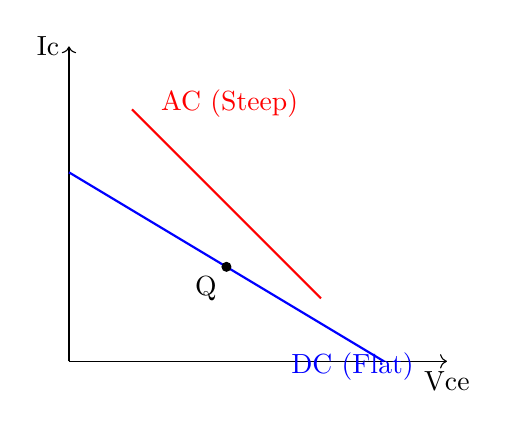
\begin{tikzpicture}[scale=0.8]
    \draw[->] (0,0) -- (0,5) node[left] {Ic};
    \draw[->] (0,0) -- (6,0) node[below] {Vce};
    
    % DC Load line
    \draw [thick, blue] (0, 3) -- (5, 0) node[pos=0.9, below] {DC (Flat)};
    % AC Load line
    \draw [thick, red] (1, 4) -- (4, 1) node[pos=0.1, above right] {AC (Steep)};
    
    \filldraw (2.5, 1.5) circle (2pt) node[below left] {Q};
\end{tikzpicture}
\end{center}

\textbf{AC Load Line Characteristics:}

\begin{itemize}
    \item \textbf{Definition}: Represents dynamic operation during signal amplification
    \item \textbf{Equation}: $i_c = \frac{V_{CC}-V_{CEQ}}{R'_c} - \frac{v_{ce}}{R'_c}$ where $R'_c = RC||RL$
    \item \textbf{Comparison with DC load line}:
      \begin{itemize}
        \item AC load line is steeper than DC load line
        \item Passes through Q-point
        \item Determines voltage and current signal swings
      \end{itemize}
    \item \textbf{Significance}: Defines maximum undistorted output signal
    \item \textbf{Limiting factor}: Avoiding saturation and cutoff regions
\end{itemize}

\begin{mnemonicbox}AC Amplitude Controlled by Load line Angle\end{mnemonicbox}
\end{solutionbox}

\questionmarks{3(a)}{3}{Draw the fixed bias circuit and explain working of it}

\begin{solutionbox}
\begin{center}
\begin{circuitikz}[american]
    \draw (0,0) node[npn] (q) {};
    \draw (q.E) -- ++(0,-0.5) node[ground] {};
    
    % Base Resistor
    \draw (q.B) -- ++(-1.5,0) coordinate (b) to[R, l=$R_B$, -*] (b |- q.C) coordinate (top);
    
    % Collector Resistor
    \draw (top) -- (q.C);
    \draw (top) to[R, l=$R_C$, -o] ++(0,1.5) node[above] {$V_{CC}$};
    \draw (q.C) to[short, *-o] ++(1,0) node[right] {Output};
    \draw (q.B) to[short, -o] ++(-2,0) node[left] {Input};
\end{circuitikz}
\end{center}

\begin{itemize}
    \item \textbf{Structure}: Base resistor connected to VCC, collector resistor for load
    \item \textbf{Operation}: Fixed base current biases transistor
    \item \textbf{Disadvantage}: Poor stability against temperature changes
\end{itemize}

\begin{mnemonicbox}Fixed Bias Feeds Base from power supply\end{mnemonicbox}
\end{solutionbox}

\questionmarks{3(b)}{4}{In hartley oscillator L1=5mH, L2=10mH, C=0.01$\mu$F. Calculate frequency of oscillations.}

\begin{solutionbox}
\textbf{Solution:}

\begin{itemize}
    \item \textbf{Given}: L1=5mH, L2=10mH, C=0.01$\mu$F
    \item \textbf{Frequency formula}: $f = \frac{1}{2\pi\sqrt{C(L1+L2)}}$
    \item \textbf{Calculation}:
      \begin{itemize}
        \item Total inductance LT = L1 + L2 = 5mH + 10mH = 15mH = 15$\times10^{-3}$ H
        \item C = 0.01$\mu$F = 1$\times10^{-8}$ F
        \item $f = \frac{1}{2\pi\sqrt{15\times10^{-3} \times 1\times10^{-8}}}$
        \item $f = \frac{1}{2\pi\sqrt{15\times10^{-11}}}$
        \item $f = \frac{1}{2\pi \times 3.873 \times 10^{-6}}$
        \item $f = \frac{1}{24.33 \times 10^{-6}}$
        \item $f = 41,101 \text{ Hz} \approx 41.1 \text{ kHz}$
      \end{itemize}
\end{itemize}

\begin{mnemonicbox}For Hartley's frequency, add coils then take square root\end{mnemonicbox}
\end{solutionbox}

\questionmarks{3(c)}{7}{Draw and explain the frequency response curve of two stage RC coupled amplifier.}

\begin{solutionbox}
\begin{center}
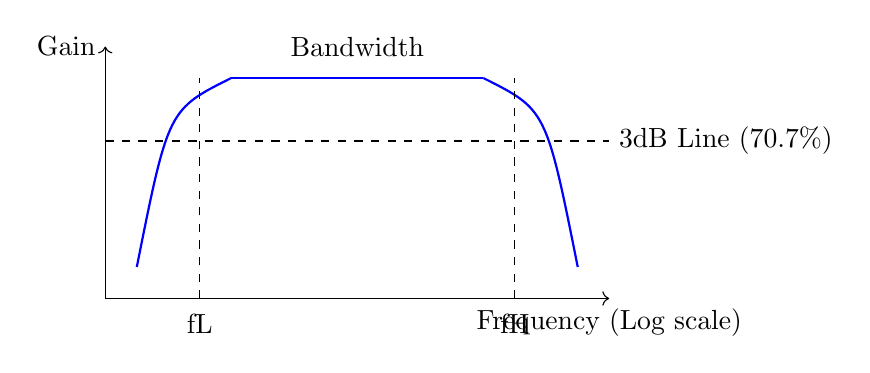
\begin{tikzpicture}[scale=0.8]
    \draw[->] (0,0) -- (0,4) node[left] {Gain};
    \draw[->] (0,0) -- (8,0) node[below] {Frequency (Log scale)};
    
    \draw [thick, blue] (0.5, 0.5) .. controls (1, 3) .. (2, 3.5); % Low Hz
    \draw [thick, blue] (2, 3.5) -- (6, 3.5); % Mid Hz
    \draw [thick, blue] (6, 3.5) .. controls (7, 3) .. (7.5, 0.5); % High Hz
    
    \draw [dashed] (0, 2.5) -- (8, 2.5) node[right] {3dB Line (70.7\%)};
    
    \draw [dashed] (1.5, 0) -- (1.5, 3.5);
    \node at (1.5, -0.4) {fL};
    
    \draw [dashed] (6.5, 0) -- (6.5, 3.5);
    \node at (6.5, -0.4) {fH};
    
    \node at (4, 4) {Bandwidth};
\end{tikzpicture}
\end{center}

\textbf{Two-Stage RC Coupled Amplifier Frequency Response:}

\begin{itemize}
    \item \textbf{Low-frequency region}: Gain rises with frequency (< 50Hz)
      \begin{itemize}
        \item Limited by coupling and bypass capacitors
      \end{itemize}
    \item \textbf{Mid-frequency region}: Constant maximum gain (50Hz-20kHz)
      \begin{itemize}
        \item Flat response, ideal operating region
      \end{itemize}
    \item \textbf{High-frequency region}: Gain drops with frequency (> 20kHz)
      \begin{itemize}
        \item Limited by transistor capacitances and Miller effect
      \end{itemize}
    
    \item \textbf{Bandwidth}: Range of frequencies with gain $\ge$ 70.7\% of maximum gain
    \item \textbf{Cutoff frequencies}: Points where gain drops by 3dB (0.707 times max gain)
\end{itemize}

\begin{mnemonicbox}Low-flat-high: capacitors block, amplify well, then roll off\end{mnemonicbox}
\end{solutionbox}

\vspace{0.5em}\centerline{\textbf{OR}}\questionmarks{3(a)}{3}{Explain in detail barkhausen criterion for oscillation.}

\begin{solutionbox}
\textbf{Barkhausen Criterion:}

\begin{center}
\captionof{table}{Conditions for Oscillation}
\begin{tabulary}{\linewidth}{|L|L|}
\hline
\textbf{Condition} & \textbf{Requirement} \\
\hline
\textbf{Loop Gain} & Must equal exactly 1 ($A\beta = 1$) \\
\hline
\textbf{Phase Shift} & Must be 0$^\circ$ or 360$^\circ$ around loop \\
\hline
\end{tabulary}
\end{center}

\begin{itemize}
    \item \textbf{Purpose}: Ensures sustained oscillations without damping
    \item \textbf{Consequences}: 
      \begin{itemize}
        \item If $A\beta < 1$: Oscillations die out
        \item If $A\beta > 1$: Oscillations grow until limited by nonlinearity
        \item If $A\beta = 1$: Stable oscillations maintained
      \end{itemize}
\end{itemize}

\begin{mnemonicbox}Barkhausen's Balance: Loop Gain=1, Phase=360$^\circ$\end{mnemonicbox}
\end{solutionbox}

\vspace{0.5em}\centerline{\textbf{OR}}\questionmarks{3(b)}{4}{Explain the effect of negative feedback on the gain of amplifier}

\begin{solutionbox}
\textbf{Effect of Negative Feedback on Amplifier Gain:}

\begin{center}
\captionof{table}{Feedback Comparison}
\begin{tabulary}{\linewidth}{|L|L|L|}
\hline
\textbf{Parameter} & \textbf{Without Feedback} & \textbf{With Feedback} \\
\hline
\textbf{Voltage Gain} & A & A/(1+A$\beta$) \\
\hline
\textbf{Stability} & Less stable & More stable \\
\hline
\textbf{Bandwidth} & Lower & Higher \\
\hline
\textbf{Distortion} & Higher & Lower \\
\hline
\end{tabulary}
\end{center}

\begin{itemize}
    \item \textbf{Gain reduction}: Gain decreases by factor (1+A$\beta$)
    \item \textbf{Gain-bandwidth tradeoff}: Bandwidth increases as gain decreases
    \item \textbf{Gain stabilization}: Less affected by temperature and component variations
\end{itemize}

\begin{mnemonicbox}Negative Feedback: Less Gain, More Stability\end{mnemonicbox}
\end{solutionbox}

\vspace{0.5em}\centerline{\textbf{OR}}\questionmarks{3(c)}{7}{Draw fan regulator circuit and explain how it will control the speed of fan.}

\begin{solutionbox}
\begin{center}
\begin{circuitikz}[american]

    \draw (0,0) to[sV, l=AC] (0,4) -- (3,4);
    \draw (3,4) to[L, l=Fan] (6,4);
    
    % Triac vertical
    % mirror puts gate on left for vertical/downward path?
    % Verify: standard triac gate is to the right. Mirror puts it left.
    \draw (6,4) to[triac, n=T, mirror] (6,0) -- (0,0);
    
    % Trigger circuit
    \draw (3,4) -- (3,2) to[vR, l=$R$] (3,0.5) to[C, l=$C$] (6,0.5) -- (6,0);
    
    % Diac
    % Connect to Gate
    \draw (3, 0.5) to[generic, l=DIAC, n=D] (T.gate);
\end{circuitikz}
\end{center}

\textbf{Fan Regulator Operation:}

\begin{itemize}
    \item \textbf{Control method}: Phase angle control using TRIAC and DIAC
    \item \textbf{Working principle}: RC network creates variable phase shift
    \item \textbf{Speed control}: Variable resistor adjusts RC time constant
    \item \textbf{Operation sequence}:
      \begin{itemize}
        \item RC network delays DIAC firing
        \item DIAC triggers TRIAC at adjustable point in AC cycle
        \item TRIAC conducts for remaining portion of AC half-cycle
        \item Less conduction time = lower power to fan = slower speed
      \end{itemize}
    \item \textbf{Advantages}: Simple design, smooth control, energy efficient
    \item \textbf{Applications}: Ceiling fans, exhaust fans, cooling systems
\end{itemize}

\begin{mnemonicbox}Delay the TRIAC firing, control fan's speed\end{mnemonicbox}
\end{solutionbox}

\questionmarks{4(a)}{3}{Write short note on natural commutation}

\begin{solutionbox}
\textbf{Natural Commutation:}

\begin{itemize}
    \item \textbf{Definition}: SCR turns off automatically when current falls below holding current
    \item \textbf{Process}: Occurs in AC circuits at each zero-crossing point
    \item \textbf{Requirements}: No external components needed, inherent to AC operation
\end{itemize}

\begin{mnemonicbox}Natural Commutation: Zero Current Crossings Turn Off Thyristors\end{mnemonicbox}
\end{solutionbox}

\questionmarks{4(b)}{4}{Explain the parameters gain and bandwidth of amplifier.}

\begin{solutionbox}
\begin{center}
\captionof{table}{Amplifier Parameters}
\begin{tabulary}{\linewidth}{|L|L|L|}
\hline
\textbf{Parameter} & \textbf{Definition} & \textbf{Formula} \\
\hline
\textbf{Gain (A)} & Ratio of output to input signal & A = Vout/Vin \\
\hline
\textbf{Bandwidth (BW)} & Frequency range with gain $\ge$ 70.7\% of maximum & BW = fH - fL \\
\hline
\end{tabulary}
\end{center}

\begin{itemize}
    \item \textbf{Gain-bandwidth product}: Remains constant (GBP = Gain $\times$ Bandwidth)
    \item \textbf{Cutoff frequencies}: Lower (fL) and higher (fH) frequencies where gain drops by 3dB
    \item \textbf{Significance}: Determines amplifier's ability to handle different frequencies
\end{itemize}

\begin{mnemonicbox}Good Amplifiers Balance Width and Magnitude\end{mnemonicbox}
\end{solutionbox}

\questionmarks{4(c)}{7}{Draw the construction and characteristics of triac and describe working of it, also write the application of triac.}

\begin{solutionbox}
\begin{center}
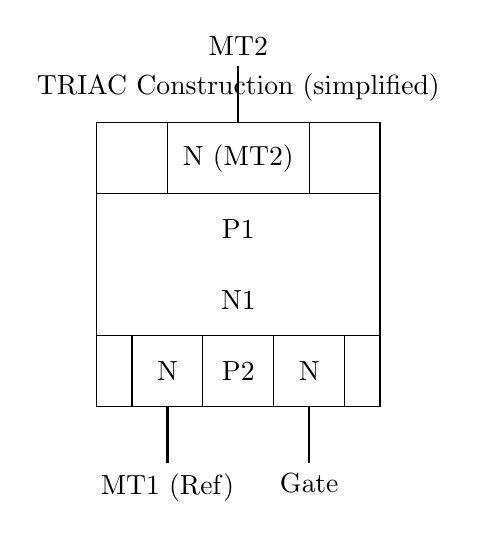
\begin{tikzpicture}[scale=0.9]
    % Construction
    \draw (0,0) rectangle (4, 4);
    \node at (2, 4.5) {TRIAC Construction (simplified)};
    
    \draw (0, 3) -- (4, 3);
    \draw (0, 1) -- (4, 1);
    
    \node at (2, 3.5) {N (MT2)};
    \draw (1, 3) -- (1, 4); \draw (3, 3) -- (3, 4);
    
    \node at (2, 2.5) {P1};
    \node at (2, 1.5) {N1};
    \node at (2, 0.5) {P2};
    
    % Gates N regions at bottom
    \draw (0.5, 0) rectangle (1.5, 1); \node at (1, 0.5) {N};
    \draw (2.5, 0) rectangle (3.5, 1); \node at (3, 0.5) {N};
    
    \draw [thick] (2, 4) -- (2, 4.8) node[above] {MT2};
    \draw [thick] (1, 0) -- (1, -0.8) node[below] {MT1 (Ref)};
    \draw [thick] (3, 0) -- (3, -0.8) node[below] {Gate};
\end{tikzpicture}
\hspace{1cm}
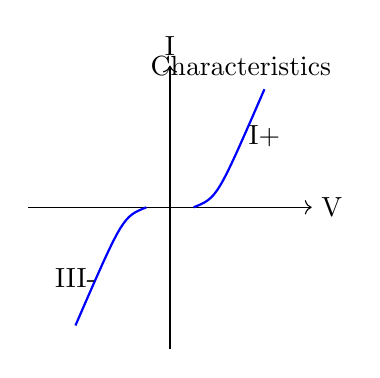
\begin{tikzpicture}[scale=0.6]
    % VI Char
    \draw[->] (-3,0) -- (3,0) node[right] {V};
    \draw[->] (0,-3) -- (0,3) node[above] {I};
    
    \draw [thick, blue] (0.5, 0) .. controls (1, 0.2) .. (2, 2.5); % Q1
    \draw [thick, blue] (-0.5, 0) .. controls (-1, -0.2) .. (-2, -2.5); % Q3
    
    \node at (2, 1.5) {I+};
    \node at (-2, -1.5) {III-};
    \node at (1.5, 3) {Characteristics};
\end{tikzpicture}
\end{center}

\textbf{TRIAC Operation:}

\begin{itemize}
    \item \textbf{Structure}: Five-layer PNPN bidirectional device
    \item \textbf{Switching}: Conducts in both directions when triggered
    \item \textbf{Triggering modes}: Four quadrant operation possible
    \item \textbf{Turn-off}: Natural commutation at current zero-crossing
\end{itemize}

\textbf{Applications:}
\begin{itemize}
    \item Light dimmers, Fan speed controllers, Heater controls, Motor speed regulation, AC power switching
\end{itemize}

\begin{mnemonicbox}TRIAC Takes AC Control in Both Directions\end{mnemonicbox}
\end{solutionbox}

\vspace{0.5em}\centerline{\textbf{OR}}\questionmarks{4(a)}{3}{Write any three application of SCR.}

\begin{solutionbox}
\textbf{Applications of SCR:}

\begin{center}
\captionof{table}{SCR Applications}
\begin{tabulary}{\linewidth}{|L|L|}
\hline
\textbf{Application} & \textbf{Function} \\
\hline
\textbf{DC Motor Speed Control} & Provides variable DC to motors \\
\hline
\textbf{Battery Chargers} & Regulates charging current \\
\hline
\textbf{Power Inverters} & Converts DC to AC efficiently \\
\hline
\end{tabulary}
\end{center}

\begin{itemize}
    \item \textbf{Advantages}: High power handling, efficient control, robust operation
    \item \textbf{Limitations}: Requires forced commutation in DC circuits
\end{itemize}

\begin{mnemonicbox}SCR Controls DC - Motors, Batteries, Inverters\end{mnemonicbox}
\end{solutionbox}

\vspace{0.5em}\centerline{\textbf{OR}}\questionmarks{4(b)}{4}{Explain holding current and latching current with reference to SCR}

\begin{solutionbox}
\begin{center}
\captionof{table}{SCR Current Parameters}
\begin{tabulary}{\linewidth}{|L|L|L|}
\hline
\textbf{Parameter} & \textbf{Definition} & \textbf{Typical Values} \\
\hline
\textbf{Holding Current (IH)} & Minimum current to maintain conduction & 5-40 mA \\
\hline
\textbf{Latching Current (IL)} & Minimum current to establish conduction & 10-100 mA \\
\hline
\end{tabulary}
\end{center}

\begin{itemize}
    \item \textbf{Latching current}: Must be exceeded briefly after triggering for SCR to latch
    \item \textbf{Holding current}: Must be maintained to keep SCR in conduction
    \item \textbf{Relationship}: Usually IL > IH
    \item \textbf{Significance}: Critical for reliable switching operation
\end{itemize}

\begin{mnemonicbox}Latch with more, Hold with less, both keep SCR conducting\end{mnemonicbox}
\end{solutionbox}

\vspace{0.5em}\centerline{\textbf{OR}}\questionmarks{4(c)}{7}{Draw and explain in detail block diagram of operational amplifier.}

\begin{solutionbox}
\begin{center}
\begin{tikzpicture}[gtu block]
    \node (diff) [draw, rectangle, align=center, minimum height=1.5cm] {1. Input\\Differential\\Stage};
    \node (mid) [draw, rectangle, align=center, right=1cm of diff, minimum height=1.5cm] {2. Intermediate\\Stage};
    \node (out) [draw, rectangle, align=center, right=1cm of mid, minimum height=1.5cm] {3. Output\\Stage};
    
    \node (bias) [draw, rectangle, align=center, below=1cm of mid] {Bias Circuit};
    \node (comp) [draw, rectangle, align=center, above=1cm of mid] {Frequency\\Compensation};
    
    \draw [gtu arrow] (diff) -- (mid);
    \draw [gtu arrow] (mid) -- (out);
    \draw [gtu arrow] (mid) -- (comp);
    \draw [gtu arrow] (bias) -| (diff);
    \draw [gtu arrow] (bias) -- (mid);
    \draw [gtu arrow] (bias) -| (out);
    
    \node [left=0.5cm of diff] {Input};
    \draw [gtu arrow] (diff.west) +(-0.5, 0.3) -- (diff.west |- 0, 0.3);
    
    \node [right=0.5cm of out] {Output};
    \draw [gtu arrow] (out) -- +(1.5, 0);
\end{tikzpicture}
\end{center}

\textbf{Op-Amp Blocks and Functions:}

\begin{itemize}
    \item \textbf{Input differential stage}: High input impedance, Rejects common-mode signals, Provides differential voltage gain
    \item \textbf{Intermediate stage}: Additional voltage gain, Level shifting, Frequency compensation
    \item \textbf{Output stage}: Low output impedance, Current amplification, Power capability for driving loads
    \item \textbf{Bias circuit}: Establishes proper operating points, Temperature stability
    \item \textbf{Frequency compensation}: Prevents oscillation, Controls frequency response
\end{itemize}

\begin{mnemonicbox}Differential Input, Gain in Middle, Power at Output\end{mnemonicbox}
\end{solutionbox}

\questionmarks{5(a)}{3}{Draw and explain in brief inverting amplifier.}

\begin{solutionbox}
\begin{center}
\begin{circuitikz}[american]
    \draw (5,0) node[op amp] (opamp) {};
    
    % Feedback
    \draw (opamp.-) -- ++(0,1.5) coordinate (tmp) to[R, l=$R_f$] (tmp -| opamp.out) -- (opamp.out);
    
    % Input
    \draw (opamp.-) to[R, l=$R_{in}$, -o] (-1, 0.5) node[left] {$V_{in}$};
    
    % Ground
    \draw (opamp.+) -- ++(0,-0.5) node[ground] {};
    
    % Output
    \draw (opamp.out) to[short, -o] ++(1,0) node[right] {$V_{out}$};
\end{circuitikz}
\end{center}

\begin{itemize}
    \item \textbf{Gain formula}: Vout = -(Rf/Rin) $\times$ Vin
    \item \textbf{Operation}: Input signal inverted with amplification
    \item \textbf{Virtual ground}: Inverting input maintained at 0V
\end{itemize}

\begin{mnemonicbox}Inverting means Negative Gain equals -Rf/Rin\end{mnemonicbox}
\end{solutionbox}

\questionmarks{5(b)}{4}{Draw and explain the block diagram of regulated power supply.}

\begin{solutionbox}
\begin{center}
\begin{tikzpicture}[gtu block]
    \node (xform) [draw, rectangle, minimum height=1cm] {Transformer};
    \node (rect) [draw, rectangle, minimum height=1cm, right=0.5cm of xform] {Rectifier};
    \node (filt) [draw, rectangle, minimum height=1cm, right=0.5cm of rect] {Filter};
    \node (reg) [draw, rectangle, minimum height=1cm, right=0.5cm of filt] {Regulator};
    \node (load) [right=0.5cm of reg] {RL};
    
    \draw [gtu arrow] (xform) -- (rect);
    \draw [gtu arrow] (rect) -- (filt);
    \draw [gtu arrow] (filt) -- (reg);
    \draw [gtu arrow] (reg) -- (load);
    
    \node [left=0.5cm of xform] {AC Line};
    \draw [gtu arrow] (xform.west) +(-0.5, 0) -- (xform);
\end{tikzpicture}
\end{center}

\textbf{Regulated Power Supply Stages:}

\begin{itemize}
    \item \textbf{Transformer}: Steps down AC voltage to required level
    \item \textbf{Rectifier}: Converts AC to pulsating DC (diode bridge)
    \item \textbf{Filter}: Smooths pulsating DC (capacitors)
    \item \textbf{Regulator}: Maintains constant output despite variations
\end{itemize}

\begin{mnemonicbox}Transform, Rectify, Filter, Regulate for Stable DC\end{mnemonicbox}
\end{solutionbox}

\questionmarks{5(c)}{7}{Draw and explain astable multivibrator.}

\begin{solutionbox}
\begin{center}
\begin{tikzpicture}[gtu block]
    \draw (0,0) rectangle (4,4);
    \node at (2, 2) {\textbf{555 Timer}};
    
    \node (vcc) at (2, 5) {VCC};
    \draw (2, 4) -- (2, 4.5);
    
    \node (gnd) at (2, -1) {GND};
    \draw (2, 0) -- (2, -0.5);
    
    \node (out) at (5, 2) {Output};
    \draw (4, 2) -- (out);
    
    % Charging path
    \node (r1) at (-2, 3.5) {R1};
    \node (r2) at (-2, 2) {R2};
    \node (cap) at (-2, 0) {C};
    \node [ground] at (-2, -0.5) {};
    
    \draw (vcc) -| (r1);
    \draw (r1) -- (r2);
    \draw (r2) -- (cap);
    \draw (cap) -- (-2, -0.5);
    
    % Pins
    \node [left] at (0, 3) {Discharge (7)};
    \draw (0, 3) -| (-2, 3); % Between R1 R2
    
    \node [left] at (0, 1) {Trig(2)/Thresh(6)};
    \draw (0, 1) -| (-2, 1); % Between R2 C
\end{tikzpicture}
\end{center}

\textbf{Operation of Astable Multivibrator:}

\begin{itemize}
    \item \textbf{Configuration}: Free-running oscillator with no stable states
    \item \textbf{Timing components}: External R1, R2, and C
    \item \textbf{Oscillation process}:
      \begin{itemize}
        \item Capacitor charges through R1+R2
        \item Capacitor discharges through R2
        \item Continuous charging/discharging cycle
      \end{itemize}
    \item \textbf{Frequency formula}: $f = \frac{1.44}{(R1+2R2)C}$
    \item \textbf{Output waveform}: Rectangular with duty cycle based on R1/R2 ratio
    \item \textbf{Applications}: Clock generation, LED flashers, tone generators
\end{itemize}

\begin{mnemonicbox}Always Switching, Time set by RC, Both states Least stable\end{mnemonicbox}
\end{solutionbox}

\vspace{0.5em}\centerline{\textbf{OR}}\questionmarks{5(a)}{3}{In an op amp non-inverting amplifier R1=2k$\Omega$ and Rf=200k$\Omega$. Find the voltage gain of non-inverting amplifier.}

\begin{solutionbox}
\textbf{Solution:}

\begin{itemize}
    \item \textbf{Given}: R1 = 2k$\Omega$, Rf = 200k$\Omega$
    \item \textbf{Non-inverting amplifier gain formula}: A = 1 + (Rf/R1)
    \item \textbf{Calculation}:
      \begin{itemize}
        \item A = 1 + (200k$\Omega$/2k$\Omega$)
        \item A = 1 + 100
        \item A = 101
      \end{itemize}
    \item \textbf{Result}: Voltage gain of non-inverting amplifier is 101
    \item \textbf{Significance}: Output voltage will be 101 times the input voltage
\end{itemize}

\begin{mnemonicbox}Non-inverting amplifier gain: One plus Feedback over Ground\end{mnemonicbox}
\end{solutionbox}

\vspace{0.5em}\centerline{\textbf{OR}}\questionmarks{5(b)}{4}{Draw and explain in brief circuit to get -5V regulated dc output voltage.}

\begin{solutionbox}
\begin{center}
\begin{circuitikz}[american]
    \draw (0,0) node[below] {$-V_{in}$} to[short, o-] (1,0) -- (2,0);
    \draw (2,-1) rectangle (4,1);
    \node at (3,0) {7905};
    \node [left, font=\tiny] at (2,0) {IN (2)};
    \node [right, font=\tiny] at (4,0) {OUT (3)};
    \node [above, font=\tiny] at (3,1) {GND (1)};
    
    \draw (4,0) -- (5,0) to[short, -o] (6,0) node[right] {$-5V$};
    
    \draw (1,0) to[C, l=$C_1$, *-] (1,1.5) node[ground, rotate=180] {};
    \draw (5,0) to[C, l=$C_2$, *-] (5,1.5) node[ground, rotate=180] {};
    
    \draw (3,1) -- (3,1.5) node[ground, rotate=180] {};
\end{circuitikz}
\end{center}

\textbf{Circuit Operation:}

\begin{itemize}
    \item \textbf{Key component}: 7905 negative voltage regulator IC
    \item \textbf{Input requirement}: Negative DC voltage (typically -7V to -25V)
    \item \textbf{Filtering}: Input and output capacitors for stability
    \item \textbf{Regulation method}: Series pass element with feedback control
    \item \textbf{Output characteristics}: Fixed -5V with current up to 1A
\end{itemize}

\begin{mnemonicbox}79XX for Negative, 78XX for Positive regulated voltage\end{mnemonicbox}
\end{solutionbox}

\vspace{0.5em}\centerline{\textbf{OR}}\questionmarks{5(c)}{7}{Draw and explain the block diagram of SMPS.}

\begin{solutionbox}
\begin{center}
\begin{tikzpicture}[gtu block]
    \node (emi) [draw, rectangle, align=center] {EMI\\Filter};
    \node (rect) [draw, rectangle, right=0.5cm of emi, align=center] {Rectifier\\\& Filter};
    \node (inv) [draw, rectangle, right=0.5cm of rect, align=center] {HF\\Inverter};
    \node (xform) [draw, rectangle, right=0.5cm of inv, align=center] {HF\\X-former};
    \node (outrect) [draw, rectangle, right=0.5cm of xform, align=center] {Output\\Rectifier};
    \node (out) [draw, rectangle, right=0.5cm of outrect] {DC Out};
    
    \node (ctrl) [draw, rectangle, below=1cm of inv] {Control \& Feedback};
    
    \draw [gtu arrow] (emi) -- (rect);
    \draw [gtu arrow] (rect) -- (inv);
    \draw [gtu arrow] (inv) -- (xform);
    \draw [gtu arrow] (xform) -- (outrect);
    \draw [gtu arrow] (outrect) -- (out);
    
    \draw [gtu arrow] (out.south) |- (ctrl.east);
    \draw [gtu arrow] (ctrl.north) -- (inv.south);
    
    \node [left=0.5cm of emi] {AC In};
    \draw [gtu arrow] (emi.west) +(-0.5, 0) -- (emi);
\end{tikzpicture}
\end{center}

\textbf{SMPS Operation:}

\begin{itemize}
    \item \textbf{Input stage}: Filters EMI, rectifies AC to high-voltage DC
    \item \textbf{Switching stage}: Converts DC to high-frequency AC (20-100 kHz)
    \item \textbf{Transformer}: Provides isolation and voltage transformation
    \item \textbf{Output stage}: Rectifies and filters to produce clean DC
    \item \textbf{Feedback control}: Regulates output by adjusting switching duty cycle
\end{itemize}

\textbf{Advantages of SMPS:}
\begin{itemize}
    \item \textbf{High efficiency} (80-90\%) due to switching operation
    \item \textbf{Small size and weight} from high-frequency transformer
    \item \textbf{Wide input voltage range} with stable output
    \item \textbf{Multiple output voltages} possible from single transformer
\end{itemize}

\begin{mnemonicbox}Switching Efficiently Reduces Size\end{mnemonicbox}
\end{solutionbox}

\end{document}
